\chapter{Theoretical Framework}
\begin{chapabstract}
\par A theoretical framework for elementary particles is introduced and discussed 
in detail in this chapter, in the form of the Standard Model (SM).
Fundamental particles that the SM predicts are presented, along with their quantum numbers and other properties. 
SM is formally constructed from concepts borrowed from relativistic and quantum theories.  
Motivation for the existence of a neutral Higgs boson is introduced from  
spontaneous symmetry breaking. Supersymmetry is presented as a possible solution to one of the 
hierarchy problem. Through this lens, a family of Higgs bosons is presented in 
the Two-Higgs Doblet Model (2HDM), an extension of the Standard Model; 
the charged Higgs boson (\Hpm) is presented as a member of this family. 
Finally, diffractive production\footnote{Diffractive production is also referred to as 
exclusive production in this thesis.} of the neutral SM Higgs is explored in the context of 
proton-proton scattering experiments.  
\end{chapabstract}
\label{theory}

\section{The Standard Model}
\label{sec:sm}
\subsection{Overview of the Standard Model}
\par Elementary particles in the SM are classified into {\it fermions} 
and {\it bosons}. Fermions are grouped into leptons and quarks, all of which are  
spin-$1/2$. All elementary bosons are spin-1, except for the Higgs boson which is    
spin-0. The bosons mediate interaction between the fermions by transmitting and 
conserving quantum numbers. Each 
quark and lepton has an antiparticle, which has the same mass as the original particle 
but different quantum numbers.

\par Leptons and quarks are each grouped into 3 generations, totalling 6 
fermion generations. Leptons (or quarks) in a generation have the same quantum 
numbers as the other generations, but different masses. The lightest lepton generation 
is made of the {\it electron} $(e)$ and its neutrino $(\nu_e)$. The heaviest lepton generation 
comprises the {\it tau} $(\tau))$ and its neutrino $(\nu_\tau)$, the $\tau$ lepton 
being heavier than the $e$ by 3 orders of magnitude. The lightest quark 
generation is made of the {\it up} $(u)$ and {\it down} $(d)$ quarks  
while the heaviest is made up of the {\it top} $(t)$ and {\it bottom} $(b)$ quarks -- 
the $t$ is about 90000 times heavier than the $u$. 
In the SM neutrinos are assumed to be massless but recent experimental observations 
of their oscillation have confirmed that they have non-zero mass~\cite{Fukuda:1998mi}.
These observations have set an upper bound of 2~\eV\ on the masses of each of the 
neutrinos. Table~\ref{tab:fermions} lists the properties of these neutrinos and other fermions.   

\begin{table}[!h]
\begin{center}
\begin{tabular}{|l|ccccc|}
\hline
           								& Generation                & Name      & Symbol & Electric Charge  & Mass \\
\hline\hline
\multirow{8}{*}{{\bf Leptons}}  &  \multirow{2}{*}{First}		& Electron  & $e$    & -1  & 0.5~\MeV \\
													& 								& Electron Neutrino   & $\nu_e$&  0  & $<2~\eV$ \\
					& & & & & \\
													& \multirow{2}{*}{Second} & Muon   & $\mu$  & -1 & 105.7~\MeV \\
													& 								& Muon Neutrino      & $\nu_\mu$ & 0 & $<2~\eV$ \\
					& & & & & \\
													& \multirow{2}{*}{Third} & Tau  & $\tau$  & -1 & 1.8~\GeV \\
													& 								& Tau Neutrino      & $\nu_\tau$ & 0 & $<2~\eV$ \\
\hline
					& & & & & \\
\multirow{8}{*}{{\bf Quarks}}  &  \multirow{2}{*}{First}		& Up  & $u$  & +2/3  & 2.3~\MeV \\
													& 								& Down          & $d$  & -1/3  & 4.8~\MeV \\
					& & & & & \\
													& \multirow{2}{*}{Second} & Charm & $c$  & +2/3  & 1.3~\GeV \\
													& 								& Strange       & $s$  & -1/3  & 95~\MeV \\
					& & & & & \\
													& \multirow{2}{*}{Third} & Top    & $t$  & +2/3  & 173.5~\GeV \\
													& 								& Bottom        & $b$  & -1/3  & 4.65~\GeV \\
\hline
\end{tabular}
\end{center}
\caption{A list of fermions and their properties.}
\label{tab:fermions}
\end{table}

\par There are 4 types of interactions in nature, mediated by 4 types of forces. All of them are included in the SM 
except for the gravitational force. The strength of the gravitational force
 is proportional to the product of the masses of the interacting 
particles. At the scale of elementary particle masses, the strength of gravity can be assummed to be negligible 
compared to the strength of any of the other three types of interactions. 
The \Wplus\ boson mediates the {\it weak} force, and the \Wminus\ is its antiparticle. 
These bosons are massive and carry a positive and negative electric charge respectively. 
The \Zboson\ also mediates the weak force. It is massive and carries no electric charge.  
The {\it photon} $(\gamma)$ mediates the {\it electromagnetic} force, and it is its own antiparticle. It 
is massless and carries no electric charge. 
The \Zboson, \Wpm\ and $\gamma$ bosons can interact with each other.  
The electromagnetic and weak forces are therefore combined into the {\it electro-weak} force. 
There are 8 {\it gluons} $(g)$ that mediate the {\it strong} force. Each is massless and carries two units of 
the {\it color} charge -- one is positive and the other is negative. A unit color charge can 
be either blue, red or green.  
Since the gluons can exchange color, they can also interact among themselves.

\par The {\it Higgs} boson is a quantum of the Higgs field, which is due to the Higgs mechanism. 
The Higgs field gives masses to the massive bosons 
described in the preceding paragraph, and all the fermions. The Higgs boson is spin-0, and does not 
carry any electric charge. 

\par Table~\ref{tab:bosons} lists all the bosons described above and their properties.

\begin{table}[!h]
\begin{center}
\begin{tabular}{|l|cccc|}
\hline
Interaction Type 								       & Symbol   & Multiplicity  & Electric Charge  & Mass \\
\hline\hline
\multirow{2}{*}{Weak}  &  \Wpm    &  2  					& $\pm 1$  & 91.2~\GeV \\
													   &  \Zboson &  1            & 0        & 80.4~\GeV \\
					& & & & \\
Electromagnetic  						 &$\gamma$  & 1 & 0  &  0 \\
					& & & & \\
Strong  										 & $g$  		& 8 & 0  &  0 \\
					& & & & \\
Mass 												 & $H$			& 1 & 0  & 125.4~\GeV \\
\hline
\end{tabular}
\end{center}
\caption{List of bosons. `Multiplicity' column is the number of types that a boson appears as. A gluon appears in 
8 forms of different color-anticolor combinations. The gluon is the only boson that has a color charge.}
\label{tab:bosons}
\end{table}

\par The SM has successfully predicted many particles. Most recently, the Higgs boson was discovered by scattering 
experiments at the Large Hadron Collider using the ATLAS
 and CMS detectors~\cite{HIGG-2014-14}, after it was added to the SM 
over 50 years ago. In 1983, evidence for \Wpm\ and \Zboson\ bosons was observed using data from 
the UA1~\cite{ARNISON1983103} and UA2 experiments~\cite{Banner1983476}. Gluons were discovered by the 
TASSO~\cite{Brandelik:1979bd} and PETA~\cite{PhysRevLett.43.830} collaborations in 1979. While the top 
quark was discovered rather late, in 1995 at Fermilab~\cite{Campagnari:1996ai} near Chicago, 
the charm and bottom quarks were indirectly discovered in the 1970s.

\par Some of the SM's shortfalls have already been hinted in the preceding 
paragraphs. One of the most glaring shortfall is that the SM does not include 
the gravitational force. It also predicts neutrinos to be massless, while several 
experiments have placed lower limits on their masses. The hierarchy problem, which motivates 
some of the work done for this thesis, has also not been fixed by the SM. 
Stated simply, it is unsettling that the weak force is $10^{24}$ times as heavy as 
the gravitational force. This discrepancy has undesired effects on the size of the  
Higgs field strength. This thesis sheds more light on the possibility of super-symmetry 
as a solution to this problem.    

\subsection{Building the Standard Model}
\par In natural units,\footnote{Natural units dictate that 
$c=\hbar=1$. See Chapter~\ref{intro}} the SM represents fermions and bosons by fields $\psi$ that are 
functions of space-time $x = (t,\vec{x})$. These fields' kinetic and potential energies
 are in turn represented by a Lagrangian that 
operates on them -- the Lagrangian is made up of kinetic and potential terms. Transformation of  
fields is governed by symmetries. The Lagrangian is required to be 
invariant upon several symmetry transformations. 

\par Probabilities of particle interactions have been 
shown to diverge in some limiting cases of energy and distance~\cite{1995math6202G}.
This undesirable behavior is kept in check 
by renormalizing the model at meaningful energy and distance scales~\cite{Krasnikov:1996jq}.
After renormalization schemes have been applied the SM Lagrangian can be separated into a 
component responsible for the strong and electroweak interactions. Here, the electromagnetic 
and weak interactions have been combined into the electroweak interaction (EWK); reasons 
will become clearer as the SM takes shape. Since the strong interaction is facilitated by 
color exchanges, its component is called the {\it Quantum Chromodynamics (QCD)} term.
%~\footnote{The word `chromo-' 
%has its roots in the Greek word for `color'}.  
Overall, the SM Lagrangian can be written compactly as 

\begin{equation}
\mathcal{L}_{SM} = \mathcal{L}^{QCD} + \mathcal{L}^{EWK}.
\end{equation} 
  
\subsubsection{Quantum Chromodynamics (QCD)}
\label{sec:qcdTheory}
\par As mentioned before, quarks and gluons carry a charge called color. This charge can take 
either of 3 states: red, green or blue. Conservation 
of this charge dictates the behavior of quarks and gluons. $SU(3)_C$, the multiplictive group of 
all unitary transformations in the color space, is the simplest group that represents rotations. 
$\mathcal{L}^{QCD}$ is required to be invariant under $SU(3)_C$ symmetry transformations. 
The generators of the group are the 8 $3\times 3$ hermitian matrices denoted by $\lambda_a/2$. 
%for $a\in[1,8]$. Thus, the $SU(3)$ matrix is written in the form 
%
%\begin{equation}
%U = \exp\left ( i\sum_a\theta^a\frac{\lambda^a}{2}\right ).
%\end{equation}
For quarks represented by the scalar fields $\psi(x)$ the Lagrangian  

\begin{equation}
\mathcal{L}_{\text{q}} = i\overline{\psi}(x)\gamma^{\mu}D_\mu\psi(x), 
\label{eq:freeQCD}
\end{equation}
where the $\gamma^{\mu}$ are the Dirac $\gamma$-matrices, is invariant under local $SU(3)$ transformations. Here,
 $D_\mu \equiv\partial_\mu + ig_{s}A_\mu^a\lambda_a/2$ where $g_{s}$ is the 
strong coupling constant\footnote{Not purely constant, as will be shown soon.}
 that is usually written as $\sqrt{4\pi\alpha_{s}}$ and $A_\mu = A_\mu^a\lambda_a/2$, a gauge field  
invariant under $SU(3)$ rotations. The gauge field $A_\mu^a$ represents a gluon with a color 
combination $a$, so terms in the Lagrangian with 
both $A_\mu^a$ and $\psi(x)$ represent 
interaction between gluons and quarks; the accompanying factors represent the coupling 
strength of such an interaction. For example, the interaction term in Equation~\ref{eq:freeQCD} can be expanded into 

\begin{equation}
\mathcal{L}_{\text{int}} = -\sqrt{4\pi\alpha_s}\left (\overline{\psi}_j(x)A_\mu^a\frac{\lambda^{ji}_a}{2}\gamma^\mu\psi_j(x)\right ) 
\end{equation}

where $\alpha_s$ has replaced $g_s$ and the $\frac{\lambda^{ji}_a}{2}$ term ensures that the quark changes 
color from $i$ to $j$ after the interaction with a gluon. Figure~\ref{fig:qgVet} illustrates this interaction 
term as a quark-gluon {\it vertex}, where $q$ represents the quark flavor.   

\begin{figure}[!h]
\centering
   \includegraphics[width=0.5\textwidth]{figures/gq.pdf}
\caption{Feynman diagram of a quark-gluon vertex}
\label{fig:qgVet}
\end{figure}

To include the propagation of gluons in space-time in the model 
a term  $\mathcal{L}_g$ is added using the field strength 
tensor $F^{\mu\nu}_a = \partial^\mu A^\nu_a - \partial^\nu A^\mu_a - \sqrt{4\pi\alpha_s}f^{abc}A^\mu_bA^\nu_c$. 
Here, $f^{abc}$ are the structure constants for the $SU(3)$ group.\footnote{These encode the commutation relations 
between the $\lambda_a/2$ matrices.} A more compact definition of the gluon propagation term is 

\begin{equation}
\mathcal{L}_g = -\frac{1}{4}F^{\mu\nu a}F_{\mu\nu a}.
\end{equation}

This term includes terms of orders two, three and four in $A_\mu^a$. Terms of order two are 
kinetic terms representing propagation of gluons in space and time. Terms of orders three and 
four represent gluon self interaction. Figures~\ref{fig:ggVeta} and \ref{fig:ggVetb} illustrate 
these interactions as gluon vertices.  

\begin{figure}[!h]
\begin{subfigure}{0.5\textwidth}
   \includegraphics[width=\textwidth]{figures/ggg.pdf}
\caption{}
\label{fig:ggVeta}
\end{subfigure} % 
\begin{subfigure}{0.5\textwidth}
   \includegraphics[width=\textwidth]{figures/g4.pdf}
\caption{}
\label{fig:ggVetb}
\end{subfigure}
\caption{Feynman diagrams of gluon-gluon vertices}
\end{figure}

\par The coupling strength $\alpha_s$ is dependent on the energy scale $\mu_R^2$ 
at which the theory is renormalized. Normally, a cutoff energy $(\Lambda_{QCD})$ above which 
the theory becomes non-pertubative is imposed as well. The 
dependence is described by 
 
\begin{equation}
\begin{aligned}
\alpha_s(\mu^2_R) = \frac{4\pi}{\beta_0\log\left ( \frac{\mu^2_R}{\Lambda_{QCD}}\right )} & \text{where } \beta_0 = \frac{33 - 2.n_f}{3},
\end{aligned}
\end{equation}  

Here, $n_f$ is the number of quark/gluon types 
taking part in the interaction. For $n_f<16$, $\alpha_s\xrightarrow{\text{large }\mu^2_R} 0$ and 
$\alpha_s\xrightarrow{\text{small }\mu^2_R} \infty$. This implies that at large enough  
energies quarks and gluons can move freely. At these energies summation of diagrams such 
as those in Figure~\ref{fig:ggVetb} can be done pertubatively, ignoring higher order diagrams.  
At low energies quarks and gluons are strongly coupled together and 
cannot move freely. In this scenario, pertubation theory is not applicable. 
This is why QCD is best studied at high energy colliders where approximations 
of these energy scales can be reached. The phenomena at these two limiting cases are known 
as {\it asymptotic freedom} and {\it confinement} respectively. Their practical treatment 
will be revisited in later chapters.   

\subsubsection{Electroweak Theory}
\par Fermions that interact through the electroweak force are grouped into left- and right-handed, 
depending on their chirality. Chirality is an intrinsic property of fermions, and it is an 
eigenvalue of the Weyl operater $\gamma_5$~\cite{2015arXiv150308956D} on the fermion fields. 
Left handed fermions are represented by field doublets 
$\psi_1(x) = \left ( \begin{smallmatrix} q \\ q^{'} \end{smallmatrix} \right )_L$ or 
$\left ( \begin{smallmatrix} \nu_l \\ l \end{smallmatrix} \right )_L$ where $q, q^{'}$ are the up and down type quarks
respectively, and $l, \nu_l$ are leptons. Right-handed fermions are singlets 
$\psi_2(x) = q_R$ or $\nu_{lR}$, and $\psi_3(x) = q^{'}_R$ or $l_R$. So, overall, all the fermions are represented 
as 

\begin{equation}
\psi(x) = \sum_{j=1}^3 \psi_j(x).
\end{equation}

$SU(2)$ is the simplest group that accommodates doublets so it is used to partly describe $\psi_1(x)$ transformations. 
Generators in this group are the weak isospin operators $\hat{I} = i\sigma_j/2$, where 
the $\sigma_j$ are the Pauli matrices with $j\in[1,3]$. $SU(2)_L$ is therefore a multiplicative group of all 
unitary rotations in the isospin space.  $U(1)$, a group of rotations in the complex space, 
 is sufficient to describe singlet transformations so it is used to describe all components of $\psi$. 
Generators of this group are the complex numbers $iY_j$, where $Y$ is the hypercharge and $j\in[1,3]$.
$U(1)_Y$ is therefore a group of rotations in the complex hypercharge space.  
The free\footnote{The term `free' is meant to describe a simple case where the fermions are not subject 
to any type of potential. Introduction of a potential to the Lagrangian leads to other interesting 
features.} Lagrangian 

\begin{equation}
\mathcal{L}_{\text{free}} = \sum_{j=1}^{3} i\overline{\psi}_j(x)\gamma^\mu D_\mu\psi_j(x) 
\label{eq:freeG}
\end{equation}

is required to be invariant under local $SU(2)_L\times U(1)_Y$ transformations. 
 The scalar fields for the 
fermions are required to transform as 

\begin{align}
\begin{split}
\psi_1(x) \rightarrow \psi^{'}_1(x) &= \exp(iY_1\beta(x))\exp(i\sigma_1\alpha(x)/2)\psi_1(x) \\
\psi_2(x) \rightarrow \psi^{'}_2(x) &= \exp(iY_2\beta(x))\psi_2(x) \\
\psi_3(x) \rightarrow \psi^{'}_3(x) &= \exp(iY_3\beta(x))\psi_3(x)
\end{split}
\end{align}

with $SU(2)_L$ imposed only on the doublets. The derivatives $D_\mu$ transform as  

\begin{align}
\begin{split}
D_\mu\psi_1(x) &= [\partial_\mu - ig\widetilde{W}_\mu(x) - ig^{'}y_1B_\mu(x)]\psi_1(x), \\
D_\mu\psi_2(x) &= [\partial_\mu - ig^{'}y_2B_\mu(x)]\psi_2(x), \\
D_\mu\psi_3(x) &= [\partial_\mu - ig^{'}y_3B_\mu(x)]\psi_3(x), 
\end{split}
\end{align}

with $\widetilde{W}_\mu(x) = \sigma_iW_\mu^{i}(x)/2$ is an $SU(2)$ matrix field.  Transformations of the 
gauge fields $B_\mu,\widetilde{W}_\mu$ are fixed for 
$D_\mu(x)\psi_j(x)$ to transform exactly like the $\psi_j(x)$.
The $g$ and $g^{'}$ parameters are the coupling constants corresponding to the $SU(2)$ and 
$U(1)$ groups respectively. 

\par Kinetic terms of the gauge fields are built from the gauge field tensors 
$B_{\mu\nu},\widetilde{W}_{\mu\nu}$ defined as 

\begin{align}
\begin{split}
B_{\mu\nu} = \partial_\mu B_\nu - \partial_\nu B_\mu, \\
\widetilde{W}_{\mu\nu} = \frac{\sigma_i}{2}\left [ \partial W_\nu^i - \partial_\nu W_\mu^i + g\epsilon^{ijk}W_\mu^j W_\nu^k \right ]  
\end{split}
\end{align}

to get 

\begin{equation}
\mathcal{L}_{kin} = -\frac{1}{4}B_{\mu\nu}B^{\mu\nu} - \frac{1}{4}W_{\mu\nu}^iW^{\mu\nu}_i.
\label{eq:lkin}
\end{equation}

Because the $W_{\mu\nu}^i$ term contains a quadratic piece, $\mathcal{L}_{kin}$ gives rise 
to cubic and quartic gauge self interactions whose coupling strengths are governed by $g$.
The full free Lagrangian is obtained by adding the $\mathcal{L}_{kin}$ term to Equation~\ref{eq:freeG} to get 

\begin{equation}
\mathcal{L}_{free} = \sum_{j=1}^{3} i\overline{\psi}_j(x)\gamma^\mu D_\mu\psi_j(x) - \frac{1}{4}B_{\mu\nu}B^{\mu\nu} - \frac{1}{4}W_{\mu\nu}^iW^{\mu\nu}_i = (D_\mu\psi)^\dagger D^\mu\psi.
\label{eq:finalFree}
\end{equation}
 
A mass term $\mathcal{L}_{mass}$ is not added because it destroys the gauge symmetries.

\par Interaction terms included in Equation~\ref{eq:finalFree} can be expanded into   

\begin{equation}
\mathcal{L}_{int} = g\overline{\psi}_1(x)\gamma^\mu\widetilde{W}_\mu\psi_1 + g^{'}B_\mu\sum_{j=1}^{3}Y_j\overline{\psi}_j\gamma^\mu\psi_j
\label{eq:int}
\end{equation}

where the term with $\widetilde{W}_\mu$ can in turn be expanded into 

\begin{equation}
\widetilde{W}_\mu = \frac{\sigma^i}{2}W^i_\mu = \frac{1}{\sqrt{2}}\begin{pmatrix} \sqrt{2}W_\mu^3 & W_\mu^\dagger \\ W_\mu & -\sqrt{2}W_\mu^3  \end{pmatrix}
\end{equation}

The term containing $\widetilde{W}_\mu$ gives rise to fermion interactions with a gauge 
boson $W_\mu = (W_\mu^1 + iW_\mu^2)/\sqrt{2}$ and its conjugate $W_\mu^\dagger$. 
These are identified as the \Wplus,\Wminus\ bosons.
To first order the Lagrangian component for the interaction of left-handed leptons
 $l,\nu_l$ and quarks $q,q^{'}$ with the \Wpm\ bosons can be expanded into 

\begin{equation}
\mathcal{L}_{W_{bosons}} = \frac{g}{2\sqrt{2}}W_\mu^\dagger\left ( q\gamma^\mu(1-\gamma_5)q^{'} + \overline{\nu}_l\gamma^\mu(1-\gamma_5)l  \right )
\end{equation} 

leading to vertices shown in Figure~\ref{fig:fermWvet}.

\begin{figure}[!h]
\begin{subfigure}{0.5\textwidth}
   \includegraphics[width=\textwidth]{figures/wqq.pdf}
\end{subfigure} % 
\begin{subfigure}{0.5\textwidth}
   \includegraphics[width=\textwidth]{figures/wlep.pdf}
\end{subfigure}
\caption{Feynman diagrams of left handed fermion-\Wpm vertices}
\label{fig:fermWvet}
\end{figure}

Linear combinations of $W_\mu^3$ and $B_\mu$ form the $Z^0$ and the $\gamma$ bosons, represented 
by $Z_\mu$ and $A_\mu$ respectively. They are also included in 
Equation~\ref{eq:int} and generalized as 

\begin{equation}
\begin{pmatrix}
A_\mu \\
Z_\mu 
\end{pmatrix}
= \begin{pmatrix}
\cos\theta_W & \sin\theta_W \\
-\sin\theta_W & \cos\theta_W
\end{pmatrix}
\begin{pmatrix}
B_\mu \\
W_\mu^3
\end{pmatrix}
\end{equation}  

Given that the electromagnetic charge operator is $Q$, that the electromagnetic charge is $e$ and $T_3 = \sigma_3/2$, the 
$A_\mu$ definition is fixed by 

\begin{equation}
\begin{aligned}
g\sin\theta_W = g^{'}\cos\theta_W = e  & \text{ and }  & Y = Q - T_3. 
\end{aligned}
\end{equation}

The first equation links the $SU(2)_L,U(1)_Y$ coupling constants to the electromagnetic coupling constant. 
The second equation fixes the fermion hypercharge, electromagnetic charge, and isospin quantum numbers. 
%where mixing between $W_\mu$ and $B_\mu$ is determined by $\theta_W$:
%
%\begin{equation}
%\begin{aligned}
%\cos\theta_W = \frac{g}{\sqrt{g^2 + g^{'2}}}  & \text{ and }  & \sin\theta_W = \frac{g^{'}}{\sqrt{g^2 + g^{'2}}}
%\end{aligned}
%\end{equation}
%
Figure~\ref{fig:neutBosFerm} illustrate the $\gamma, Z^0$ interactions with fermions, 
where $Q_f$ indicates electromagnetic charge operation on a fermion of flavor $f$.

\begin{figure}[!h]
\begin{subfigure}{0.5\textwidth}
   \includegraphics[width=\textwidth]{figures/photonFerm.pdf}
\end{subfigure} % 
\begin{subfigure}{0.5\textwidth}
   \includegraphics[width=\textwidth]{figures/zFerm.pdf}
\end{subfigure}
\caption{Feynman diagrams of fermion-\Zboson/$\gamma$ vertices}
\label{fig:neutBosFerm}
\end{figure}

Equation~\ref{eq:lkin} also generates gauge self-interactions, shown in Figure~\ref{fig:intGauge}. 

\begin{figure}[!h]
\begin{subfigure}{0.33\textwidth}
   \includegraphics[width=\textwidth]{figures/zw2.pdf}
\end{subfigure} % 
\begin{subfigure}{0.33\textwidth}
   \includegraphics[width=\textwidth]{figures/w4.pdf}
\end{subfigure}%
\begin{subfigure}{0.33\textwidth}
   \includegraphics[width=\textwidth]{figures/w2z2.pdf}
\end{subfigure} % 
\caption{Feynman diagrams showing self gauge interactions in the electroweak theory}
\label{fig:intGauge}
\end{figure}

\subsubsection{Spontaneous Symmetry Breaking (SSB) and the Higgs Mechanism}
\par As discussed earlier, the \Wpm\ and \Zboson\ gauge bosons are massive, but the theory 
built so far describes them as massless. The starting point for giving mass to these gauge bosons 
is to explore the effects of introducing an $SU(2)_L$ doublet of scalar 
fields $\phi(x) = \left (  \begin{smallmatrix} \phi^+ \\ \phi^0 \end{smallmatrix} \right )$, where the 
$\phi^0$ is the ground state, and a potential $V = - (\mu^2\phi^\dagger\phi + h(\phi^\dagger\phi)^2)$. 
The minimum of this potential is taken as the ground state of the system. This vacuum 
has to be unique. This is because all the other states are computed as pertubations from
 from the vacuum. 
The parameters $\mu,h$ are free and their boundary conditions can also be explored. 
$h<0$ represents an unphysical potential. $h>0$ and $\mu^2>0$ has a trivial minimum at $\phi = 0$.
Interesting conditions are when $h>0$ and $\mu^2<0$.
When $V$ is added to Equation~\ref{eq:finalFree}, the not-so-free Lagrangian, still 
invariant under $SU(2)_L\times U(1)_Y$ transformations, becomes 

\begin{equation}
\begin{aligned}
\mathcal{L} = \mathcal{L}_{free} + V, & \text{ where } & h>0,\mu^2<0.
\label{eq:fullL}
\end{aligned}
\end{equation}

$V$, with the free parameters restricted to conditions quoted in Equation~\ref{eq:fullL} has a ground state
$\phi^0$ with $|\braket{0|\phi^0|0}| = \sqrt{\frac{-\mu^2}{2h}} \equiv \frac{v}{\sqrt{2}}$. There is an infinite 
number of such degenerate states, each invariant under $U(1)$ rotations but no longer invariant under 
 $SU(2)_L\times U(1)_Y$. When one of these is chosen, the system is said to have acquired a vacuum 
expectation value (VEV). Here, the symmetry group that any of the ground states is invariant under, 
is denoted by $U(1)_Q$ to indicate that its generator $Q$ is different from the original hypercharge and 
 isospin generators $Y, I$. 
The $Q$ represents electromagnetic charge and it is defined as $I_3 + Y/2$.
 Since the ground state is invariant under a symmetry different 
from $\mathcal{L}$'s symmetry, $SU(2)_L\times U(1)_Y$ is said to be {\it spontaneously broken} to $U(1)_Q$.
More specifically, 3 $SU(2)_L\times U(1)_Y$ generators are broken and one $U(1)_Q$ generator is unbroken.  
This mechanism is called {\it spontaneous symmetry breaking (SSB)}. The Goldstone Theorem~\cite{PhysRevLett.4.380}
states that for every generator broken during SSB, the theory must contain 
a massless boson --  a Goldstone boson. For the SM Lagrangian, three Goldstone bosons are 
expected to appear after SSB. 

\par To generalize SSB the scalar doublet fields introduced above can be generalized as  

\begin{equation}
\phi(x) = \exp\left ( i\frac{\sigma_j}{2}\theta^j(x)\right )\frac{1}{\sqrt{2}}\begin{pmatrix} 0 \\ v + H(x) \end{pmatrix} 
\end{equation} 

where the Goldstone bosons are represented by $\theta^j(x)$. The $H(x)$ is a real scalar field. 
The $\theta^j(x)$ fields can be eliminated from the Lagrangian by choosing an appropriate orientation 
in the ground state since the fields are still invariant under $U(1)$ rotations. 
The kinetic piece of Equation~\ref{eq:fullL} becomes 

\begin{equation}
\begin{aligned}
(D_\mu\phi)^\dagger D^\mu\phi & \text{ with } D_\mu \equiv \partial_\mu - \frac{ig^{'}}{2}YB_\mu - igI_iW^i_\mu 
\end{aligned}
\end{equation} 

where $W_\mu^i$ for $i\in[1,3]$ are associated with eliminating the 3 Goldstone bosons through 
appropriate orientation adjustments and $B_\mu$ is associated with the unbroken $U(1)$ symmetry. 
Expanding this term shows that 

\begin{equation}
\begin{aligned}
W_\mu^{\pm} = \frac{W_\mu^1 \mp iW_\mu^2}{\sqrt{2}} & \text{ gain masses } M^2_{W^\pm} = \frac{1}{4}g^2v^2 \text{,} \\
M_Z^2 = \frac{M_W^2}{\cos^2\theta_W} & \text{ and } M_{\gamma} = 0. 
\end{aligned}
\end{equation}

SSB has effectively introduced masses to the massive gauge bosons and no mass to $\gamma$ 
owing to the unbroken $U(1)_Q$ symmetry. The most precise measurement of $M_{W^\pm}$ to date 
was performed using data collected by the CDF II detector: $80.385\pm 0.016~\GeV$ ~\cite{Aaltonen:2012bp}.
Similarly, the most precise measurement of $M_Z$ is a combination result from LEP 
experiments: $91.1876\pm 0.0021~\GeV$~\cite{ALEPH:2005ab}.  
Expanding the kinetic energy term shows that a new particle, 
a neutral Higgs boson corresponding to the field $H$, with mass $\sqrt{2hv}$ is introduced. 
The mechanism with which the gauge bosons gain mass and a neutral Higgs boson appears is 
called the {\it Higgs Mechanism}.

\subsection{The Higgs Boson}
\label{sec:higgsSM}
\par The mass of the Higgs boson was a free parameter in the Standard Model until July 
2012, when it was measured to be $125.09\pm0.24~\GeV$~\cite{Aad2012tfa} from data collected by LHC 
experiments. While several of its interaction modes have already been observed, 
the SM predicts that it couples to gauge bosons, at tree level or through a loop, 
and to fermions.  

%\par The Higgs boson coupling to gauge bosons has been discussed in the preceding section. 
\par Figure~\ref{fig:higgsVertgauge} shows the allowed Higgs vertices and their coupling strengths. 
For interactions with massive gauge bosons the coupling strengths are proportional to the square of the gauge boson mass. 
%So at 125~\GeV\ mass, the Higgs boson is more likely to couple to $\Zboson$ than it is to $\Wpm$.  
For interactions with fermions the coupling strengths are proportional to the fermion mass $m_f$. The
coupling strengths with fermions are called Yukawa couplings. Through SSB, fermions gain mass from interacting 
with the Higgs field.   

\begin{figure}[!h]
\centering
\begin{subfigure}{0.225\textwidth}
   \includegraphics[width=\textwidth]{figures/hz2.pdf}
\end{subfigure}%  
\begin{subfigure}{0.225\textwidth}
   \includegraphics[width=\textwidth]{figures/hw2.pdf}
\end{subfigure}% 
\begin{subfigure}{0.225\textwidth}
   \includegraphics[width=\textwidth]{figures/h2z2.pdf}
\end{subfigure} % 
\begin{subfigure}{0.225\textwidth}
   \includegraphics[width=\textwidth]{figures/h2w2.pdf}
\end{subfigure}% 
\begin{subfigure}{0.225\textwidth}
   \includegraphics[width=\textwidth]{figures/hFerm.pdf}
\end{subfigure}% 
\caption{Feynman diagrams showing SM neutral Higgs boson vertices with \Zboson\ and \Wpm}
\label{fig:higgsVertgauge}
\end{figure}

\par From the discussion in the preceding section, it is clear that the Higgs field does 
not interact with massless bosons. The Higgs boson however, couples indirectly to the massless 
bosons -- $\gamma$ and gluon. Figure~\ref{fig:higgsVertmasslessB} shows some of the one 
loop Feynman diagrams through which the Higgs boson interacts with photons and gluons. 

\begin{figure}[!h]
\centering
\begin{subfigure}{0.4\textwidth}
   \includegraphics[width=\textwidth]{figures/hgg.pdf}
\caption{}
\label{fig:higgsVertmasslessBa}
\end{subfigure}%  
\begin{subfigure}{0.4\textwidth}
   \includegraphics[width=\textwidth]{figures/hgamma.pdf}
\caption{}
\label{fig:higgsVertmasslessBb}
\end{subfigure}% 
\caption{Feynman diagrams showing SM neutral Higgs boson vertices with photons and gluons}
\label{fig:higgsVertmasslessB}
\end{figure}

\subsubsection{Production and decay of the Higgs boson in $pp$ collisions}
\label{sec:smHdecay}
\par During a $pp$ collisions the Higgs boson may be produced from gluon and quark interactions, 
through any of the vertices described above. The main production modes, where $V$ represents a $\Wpm$ or a $\Zboson$, are 
\begin{enumerate}
\item gluon fusion (ggF) : $gg\to H$; an inversion of the diagram in Figure~\ref{fig:higgsVertmasslessBa};
\item vector boson fusion (VBF) : $\qqbar\to VV\qqbar\to H\qqbar$;
\item associated production with a vector boson : $\qqbar\to VH$.
\item and associated production with top : $gg,\qqbar\to \ttbar H$; 
\end{enumerate}
The diagrams for these production modes are shown in Figure~\ref{fig:higgsProd}. Figure~\ref{fig:higgsProdcomp} shows 
distributions of cross sections for all the production modes, when the protons are collided at an energy 
of $8~\TeV$, versus the mass of the Higgs boson. For a 125~\GeV\ Higgs boson, the ggF production mode significantly dominates, followed by   
VBF. Other production modes have significantly lower cross sections. 

\begin{figure}[!h]
\centering
   \includegraphics[width=0.8\textwidth]{figures/h-prod.png}
\caption{Feynman diagrams showing SM neutral Higgs boson production modes in $pp$ collisions. Taken from Ref~\cite{Ghosh:2012ep}}
\label{fig:higgsProd}
\end{figure}

\par The Higgs boson can decay through any of the vertices discussed already. Figure~\ref{fig:higgsDeccomp} 
shows distributions of the branching fractions for these decay modes, plotted against the 
Higgs boson mass. At 125~\GeV, the most dominant decay mode is $\bbbar$, followed by $WW$. 
Although $\bbbar$ is dominant, most experiments search for the Higgs boson through the $WW$ 
decay mode because the former suffers from significantly larger backgrounds than the latter. 
As a matter of fact, the analysis presented in this text searches for evidence of the Higgs 
boson through the $WW$ decay channel. This discussion will be revisited in Chapter~\ref{exclH}.

\begin{figure}[!h]
\centering
\begin{subfigure}{0.55\textwidth}
   \includegraphics[width=\textwidth]{figures/Higgs_XS_8TeV_lx.pdf}
\caption{Cross sections}
\label{fig:higgsProdcomp}
\end{subfigure}%  
\begin{subfigure}{0.45\textwidth}
   \includegraphics[width=\textwidth]{figures/Higgs_BR_LM.eps}
\caption{Branching ratios}
\label{fig:higgsDeccomp}
\end{subfigure}% 
\caption{Plots showing distributions of expected cross sections for SM Higgs boson production modes in $pp$ collisions, and branching ratios for its 
decay modes, plotted against 
the Higgs mass. Taken from Ref~\cite{LHC:xs2016}}
\end{figure}



\section{Exclusive Particle Interactions}
\label{sec:diffPhy}
\subsection{Overview of exclusivity or diffraction}
\par $pp$ collisions can be grouped into two categories: {\it elastic} and {\it inelastic}. 
During elastic collisions the two protons scatter and emerge out of the collision intact. 
During inelastic collisions either one or both protons may dissociate after collision. Remnants of 
dissociation eventually fragment and hadronize, as discussed in detail in Section~\ref{sec:evgen}. 

\par Diffraction is a term widely used in optical experiments, where a beam of light is separated into 
its multiple components by frequency or wavelength. It is important to note that in that usage the sum of 
the components is exactly the same as the original beam of light. In $pp$ collisions, the term diffraction is 
used to refer to cases where no quantum numbers from the two protons are exchanged during the collision, 
such that the outgoing particles are just components of the incoming protons. 
More precisely, a virtual particle is exchanged during the $pp$ collision.
%, and vacuum quantum numbers are exchanged. 
Elastic processes are trivially diffractive. Inelastic processes 
may or may not be diffractive.

\par Although the $pp$ collision may be at high energy, the actual momentum exchanged during the scattering 
in diffractive processes is by comparison small. In that sense, diffractive processes fall in the `soft' 
energy regime where pertubative QCD does not apply. The Regge Theory~\cite{Costa:2012cb} was the first attempt 
at modelling this phenomenon.\footnote{It is important to note that this theory has since been replaced by QCD.}
Here, the amplitude of the diffractive scattering is given by the sum of all possible virtual exchange particles. 
The most dominant of these virtual particles in this theory is known as the {\it Pomeron}. Several models have 
since substituted this pomeron with other options. One such model is discussed in Section~\ref{sec:exclH}.

\par Inelastic diffractive processes in which one of the protons dissociates is known as Single Dissociation (SD). 
Inelastic diffractive processes in which both protons dissociate is known as Double Dissociation (DD). In this text, 
elastic, SD and DD processes are collectively referred to as {\it exclusive}. The motivation behind this 
nomenclature will become clear in Section~\ref{sec:exclH}. 

\par During an exclusive $pp$ collision photons may be exchanged. This exchange does not change 
the original quantum numbers of the colliding protons. With large enough momentum, the photons may 
interact to form a pair of \Wpm\ ($pp(\gamma\gamma)\to ppWW)$) bosons through one of the vertices shown in Figure~\ref{fig:intGauge}. 
Such a quartic gauge coupling is interesting. Efforts have been made to measure its cross section. 
This process may be elastic, SD or DD. Figure~\ref{fig:exclWW} illustrates these possibilities, where 
$X$ represents the remnants of proton dissociation.      

\begin{figure}[!h]
\begin{subfigure}{0.33\textwidth}
   \includegraphics[width=\textwidth]{figures/exclWW.pdf}
\caption{Elastic}
\end{subfigure} % 
\begin{subfigure}{0.33\textwidth}
   \includegraphics[width=\textwidth]{figures/exclWWsd.pdf}
\caption{Single Dissociative (SD)}
\end{subfigure}%
\begin{subfigure}{0.33\textwidth}
   \includegraphics[width=\textwidth]{figures/exclWWdd.pdf}
\caption{Double Dissociative (DD)}
\end{subfigure} % 
\caption{Diagrams showing exclusive processes through photon exchanges, producing a pair of \Wpm\ bosons}
\label{fig:exclWW}
\end{figure}

\par The cross section for the $pp(\gamma\gamma)\to ppWW$ process shown in Figure~\ref{fig:exclWW} is calculated using the 
equivalent photon approximation (EPA)~\cite{EPA0,EPA}. In EPA the photons are described by equivalent photon 
distributions $f(x)$. $f(x)$ is the probability of a photon that carries a fraction of proton energy $x$ to 
be emitted by the proton during the $pp$ collision. The cross section $\sigma_{pp(\gamma\gamma)\to ppWW}^{\text{EPA}}$ is 
then 

\begin{equation}
\sigma_{pp(\gamma\gamma)\to ppWW}^{\text{EPA}} = \iint f(x_1) f(x_2) \sigma_{\gamma\gamma\to WW} (m_{\gamma\gamma}^2) dx_1 dx_2 
\end{equation} 

where $m_{\gamma\gamma}$ is the center of mass energy of the two-photon system. This formulation has been used in several 
experiments to describe exclusive dilepton\footnote{Replace the \Wpm-pair with leptons in Figure~\ref{fig:exclWW}.} 
results~\cite{CDFgg,STARgg,CMSmumu,CMSee}.    

\subsection{Production of the exclusive Higgs boson}
\label{sec:exclH}
\par With enough shared momentum during a diffractive $pp$ collision, a 125~\GeV\ Standard 
Model Higgs boson (see Section~\ref{sec:higgsSM}) can be created through an exchange of either 
photons or gluons. From the production cross sections shown in Figure~\ref{fig:higgsProdcomp} the 
exchange of gluons is much more preferable than the exchange of photons. The interaction between the 
Higgs boson and the gluons is done through a top quark loop. Since exchange of gluons would 
alter the quantum numbers of the initial and final state protons, another gluon is exchanged 
during the collision to neutralize the overall color. The Feynman diagram in Fig.~\ref{fig:exclH} illustrates 
this process.
 
\begin{figure}[!h]
\centering
\includegraphics[width=0.8\linewidth]{figures/exclH.pdf}
\caption{Feynman diagram showing the production of the exclusive Higgs boson} 
\label{fig:exclH}
\end{figure}

\par The Khoze-Martin-Ryskin (KMR) model~\cite{Khoze} calculates the cross section for this process, and 
formulates it as 

\begin{equation}
\sigma_{pp(gg)\ra ppH} \propto \hat{\sigma}(gg\ra H)\left ( \int \frac{dQ^2_t}{Q^4_t}f_g(x_1, x_1^{'},Q^2_t)f_g(x_2, x_2^{'},Q^2_t)\right )^2. 
\end{equation}

Here, $\hat{\sigma}(gg\ra H)$ is the cross-section for the gluon fusion process that produces the Higgs boson. This quantity 
can be read directly from Figure~\ref{fig:higgsProdcomp}. The functions $f_g$~\cite{Martin} are the generalized gluon densities
for the finite proton size, that take into account the impact parameter. 
The variables $x_1$ and $x_2$ are the fractions of the momenta carried by the gluons that contribute 
to the production of the Higgs boson, with respect to the momenta of the 
protons $p_1$ and $p_2$. The variables $x_1^{'}$ and $x_2^{'}$ are the fractions 
of the momentum carried by the exchanged third gluon with respect to the momenta of the
protons $p_1$ and $p_2$ as shown in Fig.~\ref{fig:exclH}.
These gluon densities are integrated over the exchanged (third) gluon 
transverse momentum $Q_t$. 

\par For a 125~\GeV\ Standard Model Higgs boson in all decay modes, a total production cross-section 
of 3~fb is predicted when the protons collide at center-of-mass energy $8$~\TeV. The decay modes for the exclusive 
Higgs boson are the same as those discussed in Section~\ref{sec:smHdecay}, and the branching ratios 
are identical to those shown in Figure~\ref{fig:higgsDeccomp}. The analysis discussed in Chapter~\ref{exclH} 
conducts a search for events in which an exclusive Higgs boson is created in $pp$ collision at a center-of-mass 
energy of 8~\TeV.  

 

\section{Minimal Supersymmetric Standard Model} 
\label{sec:twohdm}
\par The hierarchy problem alluded to in Chapter~\ref{intro} induces a discrepancy in the predicted 
and observed Higgs boson masses. To match the observed Higgs mass, the SM has to be fine-tuned by 
subtracting semi-divergent terms from the Lagrangian. To reduce this fine-tuning, the 
Minimal Supersymmetric Standard Model (MSSM)~\cite{FAYET1976159} postulates that for each particle predicted by the SM 
there exists a super-partner with different quantum numbers. Adding such particles does 
reduce the level of fine-tuning required on the SM and moderates corrections to the 
Higgs mass. In this framework, the Higgs boson becomes a member of a family of Higgs 
bosons, and is referred to as $h$.\footnote{In 
preceding sections $h$ was represented by $H$. Apologies for the expected 
confusion.} In this specification, MSSM is referred to as hMSSM~\cite{Djouadi:2013uqa}.
In addition to $h$, hMSSM predicts 4 more Higgs bosons: two 
charged $H^{\pm}$, one CP-even $H$, and one CP-odd $A$. 
 
\subsection{Two-Higgs-Doublet Model}
\par One of the models that predict a family of Higgs bosons is the
Two-Higgs-Doublet Model (2HDM)~\cite{PhysRevD.8.1226}. 
The phenomenology of this model is categorized into two classes: type-I and type-II. The 
type-II model corresponds to the hMSSM. MSSM is built on two Higgs 
doublet fields 

\begin{equation}
\begin{aligned}
\phi_1 = \begin{pmatrix}\phi_1^+ \\ \phi_1^0 \end{pmatrix} &\text{  with VEV } & \langle\phi_1\rangle = \frac{v_1}{\sqrt{2}}, & \text{ and, } \\ 
\phi_2 = \begin{pmatrix}\phi_2^+ \\ \phi_2^0 \end{pmatrix} &\text{  with VEV } & \langle\phi_2\rangle = \frac{v_2e^{i\theta}}{\sqrt{2}}. &  
\end{aligned}
\label{eq:fields}
\end{equation}

In type-I 2HDM all fermions couple to one of the Higgs doublets, while in type-II up-type quarks couple to 
a different doublet from down-type quarks. Following the strategy used to construct 
SSB in the preceding section, the doublet fields can be generalized as 

\begin{equation}
\begin{aligned}
\phi_1 = \begin{pmatrix}\phi_1^+ \\ \frac{h_1 + v_1 + ig_1}{\sqrt{2}} \end{pmatrix}, \\ 
\phi_2 = \begin{pmatrix}\phi_2^+ \\ \frac{h_2 + v_2e^{i\theta} + ig_2}{\sqrt{2}} \end{pmatrix}.
\end{aligned}
\label{eq:fieldsGen}
\end{equation}

The total Lagrangian for the system is  
$\mathcal{L} = \mathcal{L}_{kin} + \mathcal{L}_{pot} + \mathcal{L}_{Yukawa}$, which is a sum 
of kinetic, potential and Yukawa terms.  $\mathcal{L}$ is required to conserve both charge and charge-parity (CP)
symmetries, just like the Lagrangian in the SM. The potential term,  $\mathcal{L}_{pot} = \braket{\phi^\dagger|V|\phi}$ 
is built by 

\begin{equation}
V = -\mu_1^2\hat{A}-\mu_2^2\hat{B}+h_1\hat{A}^2+h_2\hat{B}^2+h_3(\hat{C}^2+\hat{D}^2)+h_5\hat{A}\hat{B}
\end{equation}

where 

\begin{equation*}
\hat{A} \equiv \phi_1^\dagger\phi_1, \hat{B}\equiv\phi_2^\dagger\phi_2,\hat{C}\equiv\Re(\phi_1^\dagger\phi_2), 
\hat{D}\equiv\Im(\phi_1^\dagger\phi_2).
\end{equation*}

This potential is designed to conserve both charge and parity symmetries as well.
 The $\mu_i,h_i$ are free terms that eventually 
define the Higgs masses. From these parameters the Higgs bosons $H,h,A$ and 
$(H^{\pm})$ emerge. The studies presented in this text are concerned only with $H^{\pm}$. 
Present discussion is therefore limited to $H^{\pm}$. 
Moreover, since the 2HDM Lagrangian is invariant under charge transformations,  
$H^{\pm}$ is referred to as $H^+$, ignoring charge. 

\par In this setup both doublets can have real 
vacuum expectation values (VEVs). The ratio of these VEVs is known as  
$\tan\beta$. The entire parameter space of this Higgs sector is defined by $\tan\beta$ 
and the mass of $H^{\pm}$, $m_{H^{\pm}}$.    

\par The minimum conditions on $V$ give rise to the following solutions  
 
\begin{equation}
\centering
\begin{aligned}
v_1^2 &= \frac{h_1-h_2\pm Z_1}{2(h_1 - h_+)(h_2 - h_+)} \\
v_2^2 &= \frac{h_2-h_1\pm Z_2}{2(h_1 - h_+)(h_2 - h_+)} \\
Z_1 &= \sqrt{(h_1-h_2)^2 - 4(h_1-h_+)(h_2-h_+)
\left [ (h_+v^2-\mu_1^2)(h_+v^2-\mu_2^2)-\frac{\mu_3^4}{4}\right ]} \\
Z_2 &= \sqrt{(h_1-h_2)^2 - 4(h_2-h_+)(h_1-h_+)
\left [ (h_+v^2-\mu_2^2)(h_+v^2-\mu_1^2)-\frac{\mu_3^4}{4}\right ]} \\
\end{aligned}
\end{equation}

giving rise to the following higgs masses 

\begin{equation}
\begin{aligned}
m_{H^{\pm}}^2 &= -h_3(v_1^2 + v_2^2)+\mu_3^2\frac{v_1^2+v_2^2}{v_1v_2} \\
m_{A^{0}}^2 &= \frac{1}{2}\mu_3^2\frac{v_1^2+v_2^2}{v_1v_2} \\
\end{aligned}
\end{equation}

and 

\begin{equation}
\begin{split}
m_{H^0,h^0}^2 = h_1v_1^2 + h_2v_2^2 + \frac{1}{4}\mu_3^4(\tan\beta+\cot\beta) \\
\pm \sqrt{\left [ h_1v_1^2 - h_2v_2^2 + \frac{1}{4}\mu_3^4(\tan\beta-\cot\beta)\right ]^2  
+ \left (2v_1v_2h_+ - \frac{1}{2}\mu_3^2  \right )^2}. 
\end{split}
\end{equation}

Expanding the potential term of the Lagrangian reveals that $\Hplus$ can interact with 
other Higgs bosons in the sector,  
with a coupling strength dependent on the VEVs of the doublets, which is $\tan\beta$.

\par The kinetic term of the Lagrangian is 

\begin{equation}
\mathcal{L}_{kin} = (D_\mu\phi_1)^\dagger(D_\mu\phi_1) + (D_\mu\phi_2)^\dagger(D_\mu\phi_2)  
\end{equation}

where $D_\mu = \partial_\mu + gL_iW^i_\mu + g^{'}L_4B_\mu$. The $i$ index runs from 1 to 3.  
$L_i$ and $L_4$ are $4\times4$ matrices. Expanding this term reveals that the charged Higgs boson can also 
interact with gauge bosons, with vertices such as $\Zboson H^+H^-$. 

\par Interaction of 2HDM Higgs bosons with fermions is governed by the Yukawa term in the Lagrangian 

\begin{equation}
-\mathcal{L}_{Yukawa} = \eta_{ij}^{D}\overline{Q}_{iL}\phi_1D_{jR} + \varepsilon_{ij}^{U}\overline{Q}_{iL}i\sigma_2\phi_2U_{jR} + \text{leptonic sector} + ...
\label{eq:yk}
\end{equation}

$\eta^0_{ij},\varepsilon^0_{ij}$ are non-diagonal $3\times 3$ matrices and $i,j$ denote quark family 
indices. $\overline{Q}_{iL}$ denote the quark weak isospin left-handed doublets. $D_{jR}, U_{jR}$ denote the 
up-type and down-type weak isospin right-handed singlets respectively. The leptonic sector is similar to 
the quark sector. One Higgs doublet couples to the up-type fermions $(\phi_2)$ and the other couples to the 
down-type fermions. 

\subsection{The charged Higgs boson}
\label{sec:cHtheory}
\par Unlike the Standard Model Higgs boson mass, the charged Higgs boson mass is a free parameter 
in the 2HDM. As already mentioned, $\tan\beta$ is also a free parameter. Analyses presented in this 
text scan through the mass of the charged Higgs boson. Expanding Equation~\ref{eq:yk} reveals that 
couplings to fermions, $g_{\Hplus}(ud)$, are dependent on $\tan\beta$:

\begin{equation}
g_{\Hplus}(ud) = m_d\tan\beta(1+\gamma_5) + m_u\cot\beta(1-\gamma_5)
\end{equation} 

Figure~\ref{fig:chargedHverts} shows the allowed vertices between \Hplus\ and fermions, as 
well as with the SM Higgs boson $h$.  

\begin{figure}[!h]
\begin{subfigure}{0.33\textwidth}
   \includegraphics[width=\textwidth]{figures/chargedHq2.pdf}
\end{subfigure} % 
\begin{subfigure}{0.33\textwidth}
   \includegraphics[width=\textwidth]{figures/chargedHlep.pdf}
\end{subfigure}%
\begin{subfigure}{0.33\textwidth}
   \includegraphics[width=\textwidth]{figures/chargedHh.pdf}
\end{subfigure}%
\caption{Feynman diagrams showing tree level charged Higgs vertices}
\label{fig:chargedHverts}
\end{figure}

\subsubsection{Production \& decay in $pp$ collisions}
\par Production of the charged Higgs boson from $pp$ collisions depends on its mass, $m_{H^{+}}$.
For $m_{H^{+}}$ less than the mass of the $t$ quark, $m_t$, the dominant mode of production is 
through the \tHb\ process.  For $m_{H^{+}}$ greater than $m_t$ production of the charged Higgs 
in association with a top quark is dominant. Figure~\ref{fig:chargedFeyn} shows such tree-level 
diagrams. The most dominant process for $t$ production is $gg\rightarrow\ttbar$ (known as \ttbar);

\begin{figure}[!h]
\centering
\begin{subfigure}{0.3\textwidth}
   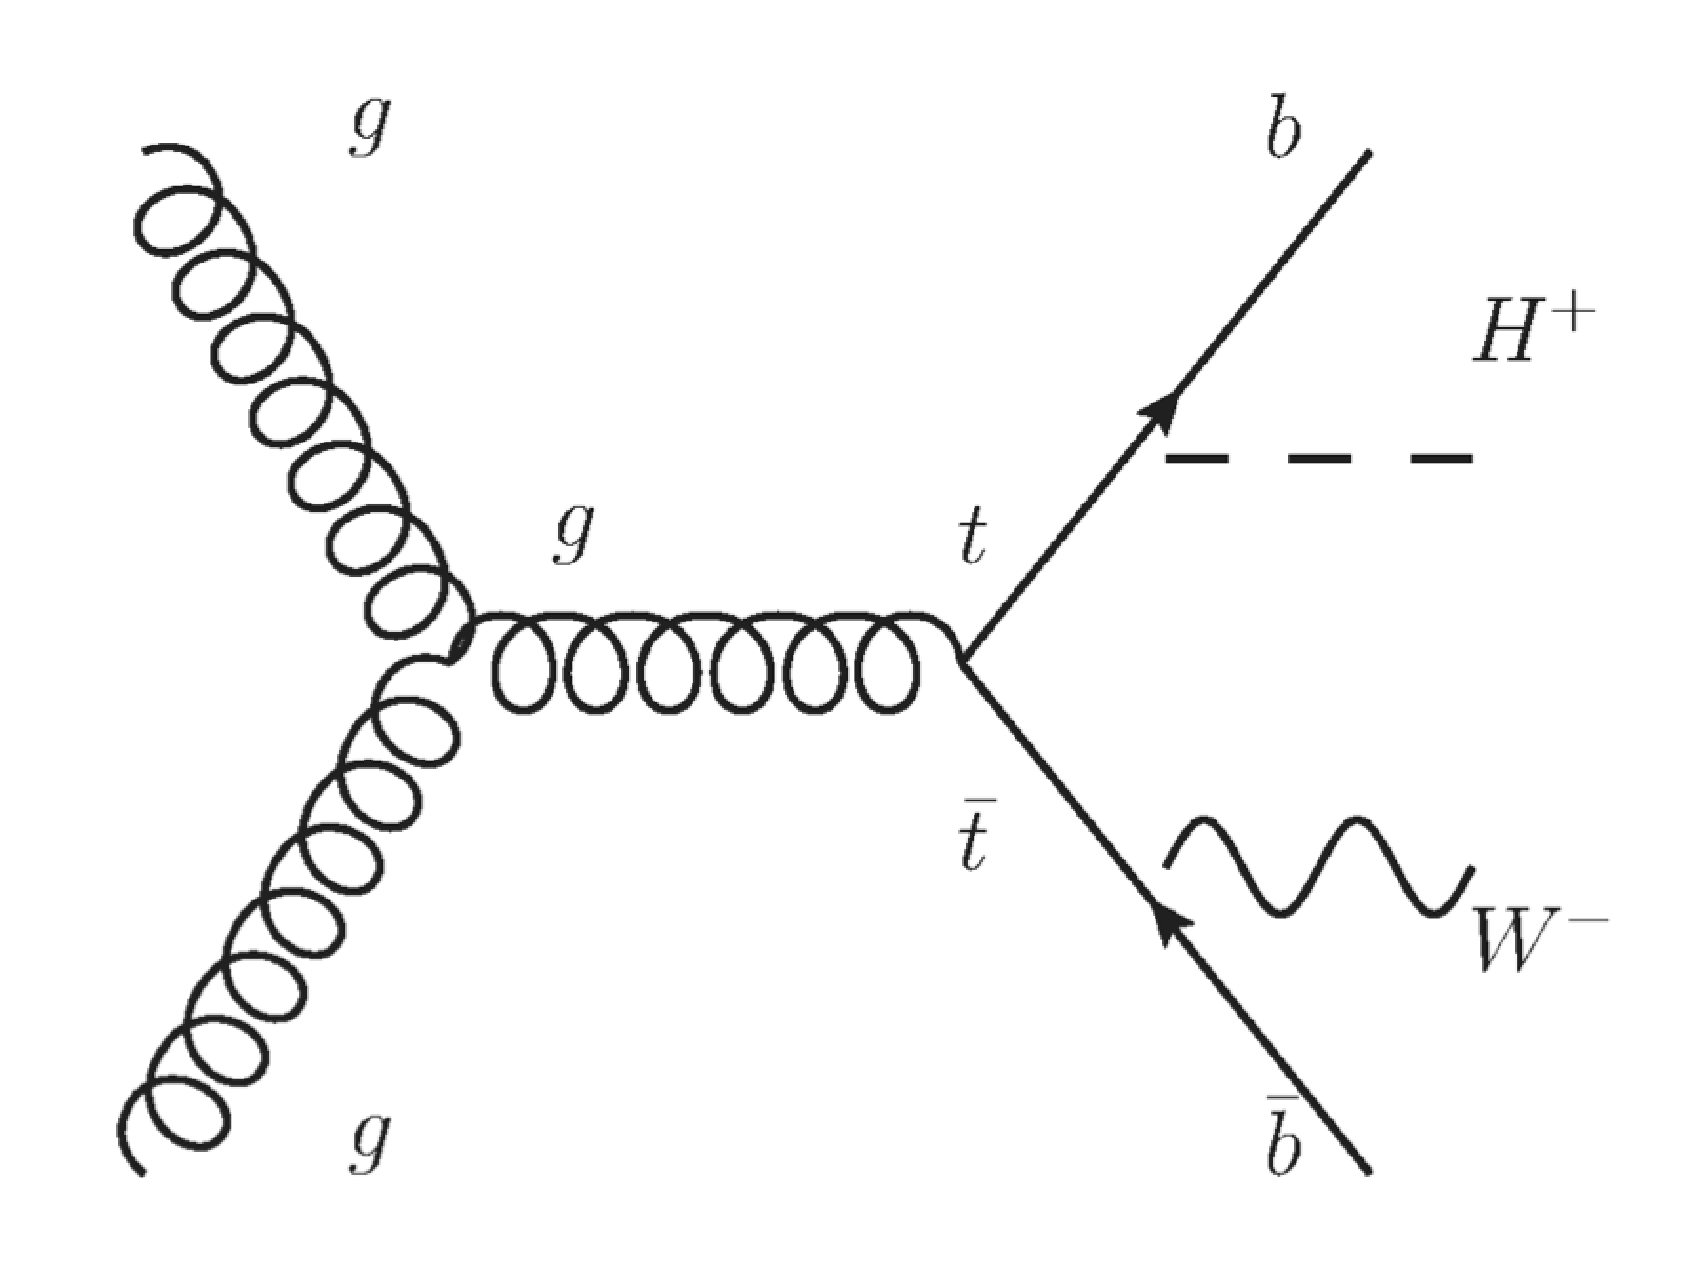
\includegraphics[width=\textwidth]{figures/feynmanIa.eps}
\caption{Top decay} 
\end{subfigure} % 
\begin{subfigure}{0.3\textwidth}
   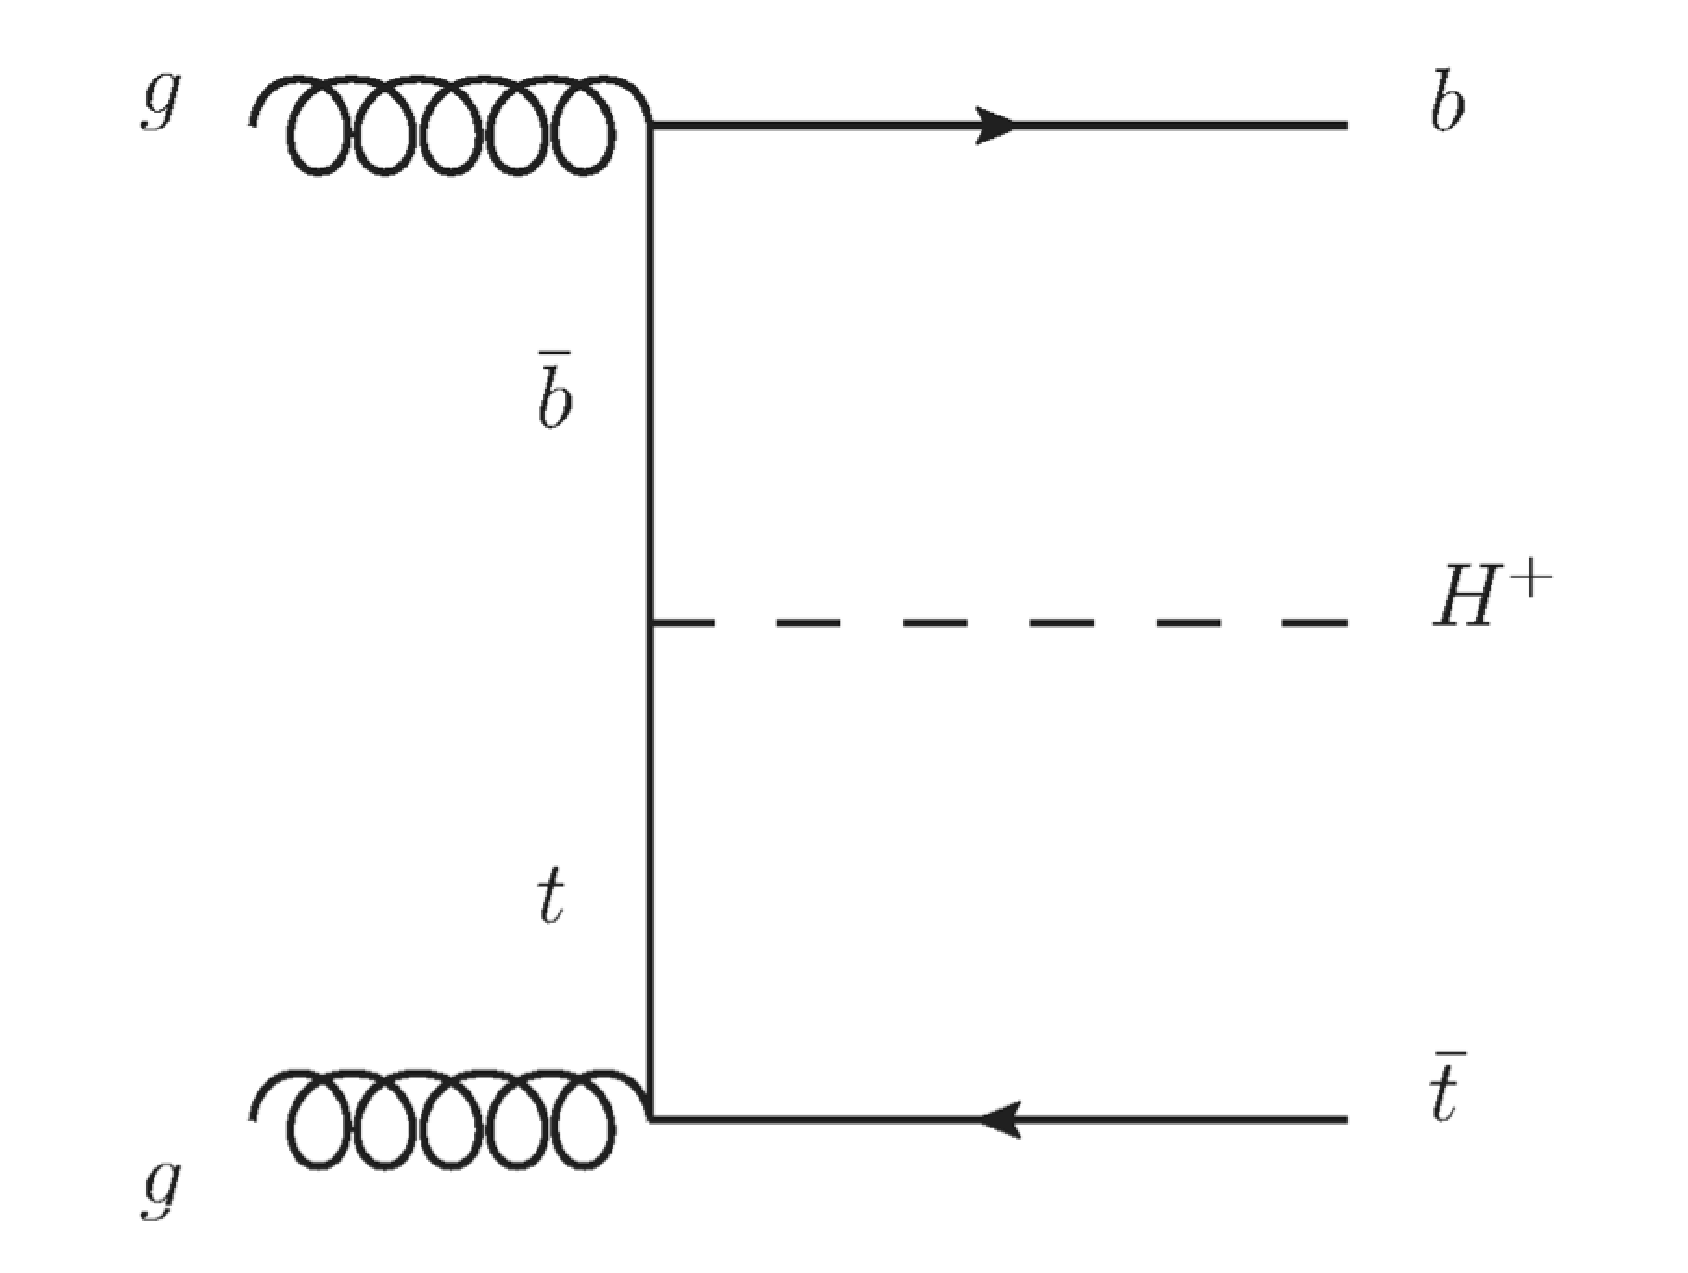
\includegraphics[width=\textwidth]{figures/feynmanIIIa.eps}
\caption{Top association -- 4FS}
\end{subfigure} % 
\begin{subfigure}{0.3\textwidth}
   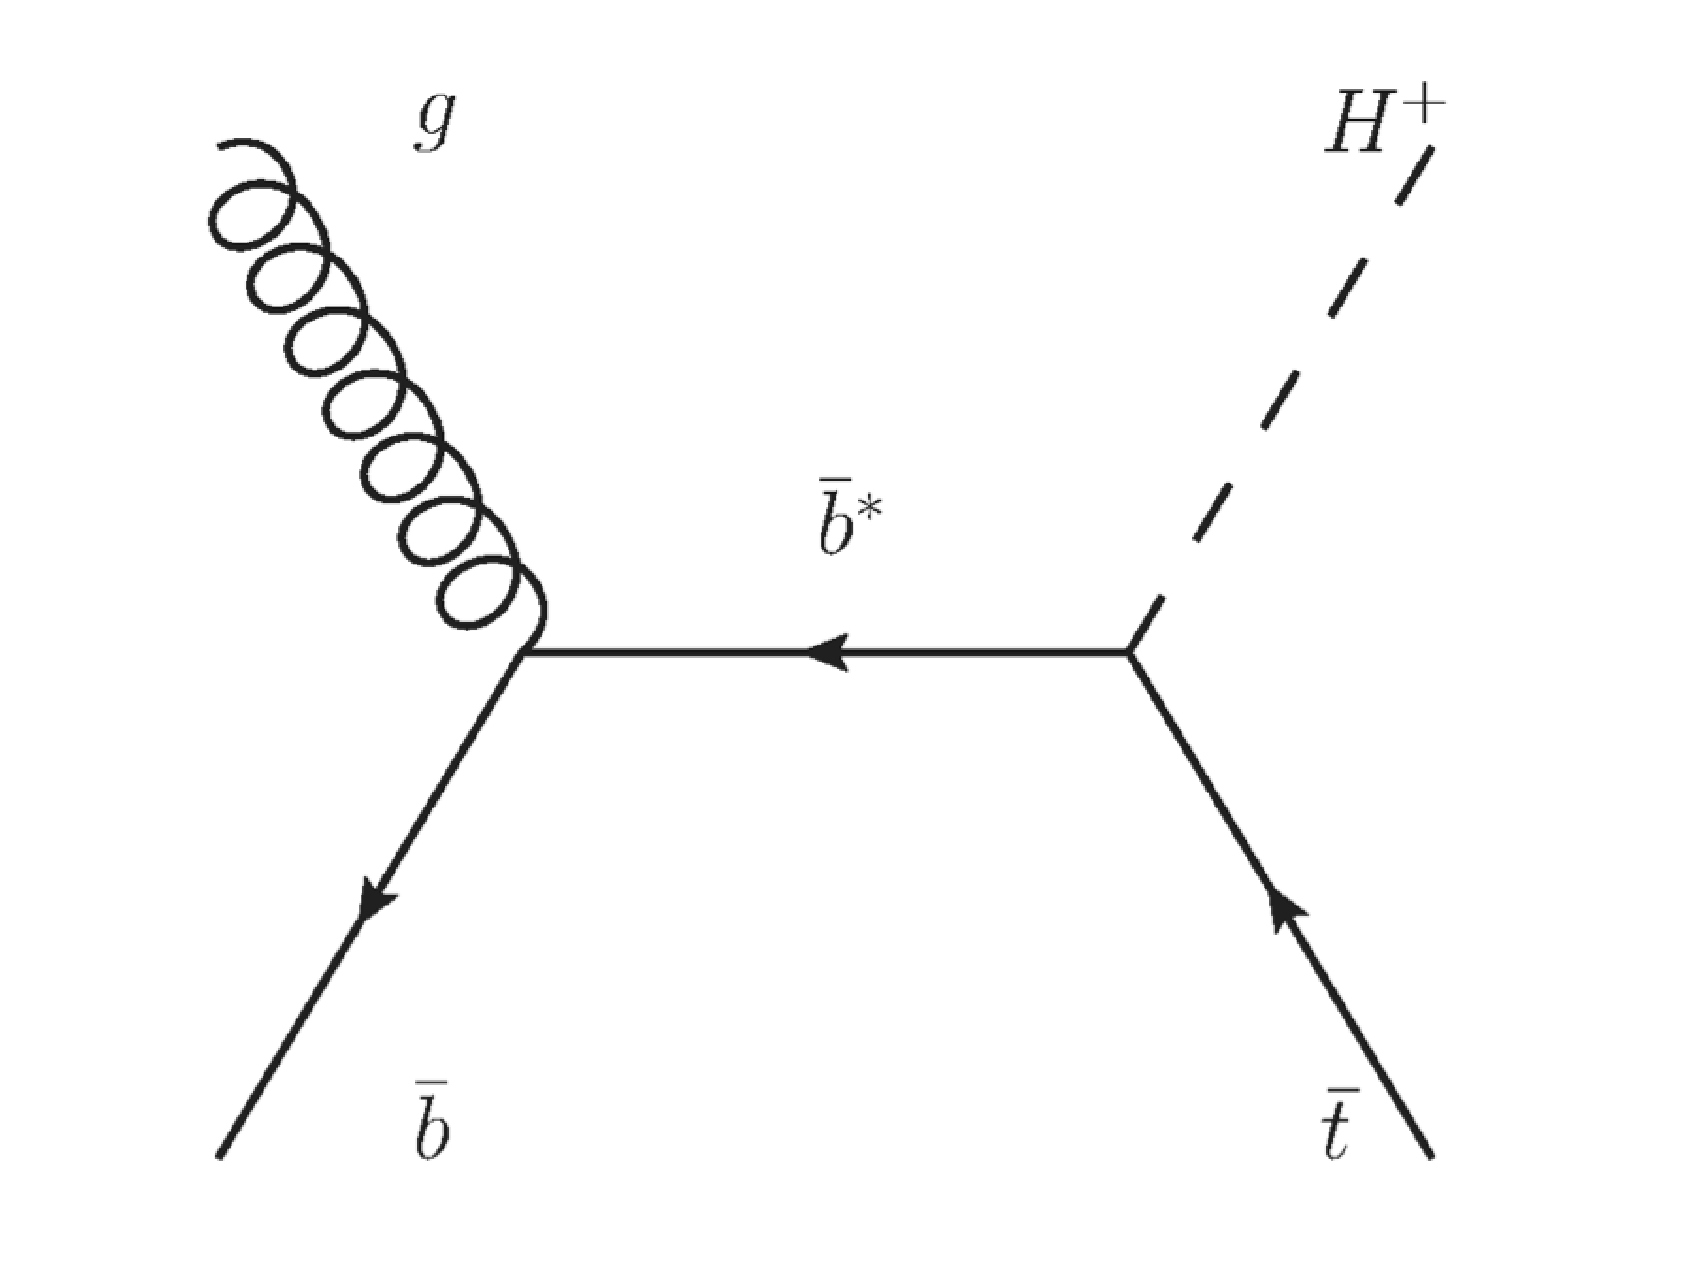
\includegraphics[width=\textwidth]{figures/feynmanIIa.eps}
\caption{Top association -- 5FS}
\end{subfigure} %
\caption{Feynman diagrams showing charged Higgs production}
\label{fig:chargedFeyn}
\end{figure}

\par For $m_{H^{+}}<m_t$ the charged Higgs is produced when one of the $t$ decays to a bottom quark. 
Clearly \ttbar\ events constitute a major background to the charged Higgs when conducting a search. 
When calculating amplitudes for these production vertices, the quark family is assummed to contain just 4
flavors of quarks $(u,d,c,s)$. The $b$ quark is included in the models only when it is necessary. 
For $m_{H^{+}}>m_t$ production can be through $gb\rightarrow tH^+$. Since the $b$ is included in this 
process, the scheme is known as the 5=flavor scheme. A 4-flavor scheme is $gg\rightarrow tbH^+$. 
Using $m_t$ as a boundary, charged Higgs bosons with mass less than 165~\GeV are referred to as {\it light}; 
those with mass greater than 200~\GeV are {\it heavy}, otherwise they are {\it intermediate}.

\par Figure~\ref{fig:chargedHxs} shows the total production cross section for a charged Higgs with 
$\mcH=200~\GeV$ plotted against $\tan\beta$, produced at $pp$ collision center-of-mass energy of $\sqs=13~\TeV$. 

\begin{figure}[h]
\centering
   \includegraphics[width=0.5\textwidth]{figures/xsec_mhp_200.pdf}
\caption{Plots of the charged Higgs production cross section against $\tan\beta$ at $\sqs=13~\TeV$ 
collision energy, for $\mcH=200~\GeV$}
\label{fig:chargedHxs}
\end{figure}

\par The \Hplus\ can decay through any of the vertices in Figure~\ref{fig:chargedHverts}. Modes 
with interactions between \Hplus\ and other Higgs bosons in the Higgs sector are very 
low, so they are ignored. Figure~\ref{fig:BR_chargedH} shows branching fractions for the significant 
decay modes for \Hplus\ in the MSSM as a function of \mcH. The $m_h^{\text{mod+}}$ alludes to the fact 
that $h$ is taken with a mass of 125~\GeV, so the branching ratios corresponds to an hMSSM scenario at 
$\tan\beta=10$ and $50$. At both $\tan\beta=10$ and 50 the dominant decay mode is $t\bbar$ for $\mcH>200~\GeV$. 
This is followed by the $\tau\nu_\tau$ mode, which is in fact more dominant at low \mcH. Due to its low 
expected background, with at least 10\% branching ratio the $\tau\nu_\tau$ mode is more attractive 
than the $t\bbar$ mode due to copious background contamination in the latter. The analysis presented 
in this text searches for evidence of \Hplus\ through the $\tau\nu_\tau$ mode. This discussion will 
be revisited in Chapter~\ref{chargedH}. 

\begin{figure}[!h]
\begin{subfigure}{0.5\textwidth}
   \includegraphics[width=\textwidth]{figures/YRHXS3_BR_fig33.eps}
\end{subfigure} % 
\begin{subfigure}{0.5\textwidth}
   \includegraphics[width=\textwidth]{figures/YRHXS3_BR_fig34.eps}
\end{subfigure}
\caption{Charged Higgs decay branching ratios in the hMSSM scenario, where $m_h^{\text{mod+}}$ alludes to 
the fact that $h$ is the observed SM Higgs. Left shows $\tan\beta=10$ and right shows $\tan\beta=50$}
\label{fig:BR_chargedH}
\end{figure}


%\begin{chapsummary}
%\par The Standard Model was presented in this chapter. First its predictions, which provide 
%the fundamental particles of nature, were outlined. Its successes and failures were outlined.
% The Standard Model was then built 
%using concepts from group theory, relativity and quantum theory. Among the Standard 
%Model predictions is the Higgs boson. Its couplings to other fundamental particles was discussed. 
%Its production in diffractive processes, in the context of proton collisions, was discussed through other models external to 
%the Standard Model, prompting motivation for one part of this thesis. The Minimal Supersymmetric Standard Model (MSSM) was introduced as a proposed 
%solution to the hierarchy problem, which the Standard Model fails to fix.  
%The MSSM predictions, such as the charged Higgs boson, were discussed. 
%The charged Higgs boson coupling to fundamental particles in the Standard Model was also outlined, 
%prompting motivation for the second part of this thesis.  
%\end{chapsummary}
